\documentclass[addpoints]{exam}

% \usepackage{fancyhdr}
\usepackage[latin1]{inputenc}
\usepackage{amsmath}
\usepackage{amsfonts}
\usepackage{amssymb}
\usepackage{graphicx}
\usepackage[hmargin=2cm,vmargin=2.5cm]{geometry}
\usepackage[normalem]{ulem}
\usepackage{enumerate}



\begin{document}

\begin{center}
	\begin{large}
		OVERVIEW
	\end{large}
\end{center}

\noindent
There are 16 problem types that address the following learning objectives. Six (6) of these are labelled as \textbf{CORE} problems:  
	\begin{description}
		\item[Problem 0] Compute limits and determine continuity and differentiability of a function given a graph or table. 
		\item[Problem 1] Find average and instantaneous rate of change in a function using the limit-based definition of the derivative. 
		\item[Problem 2 (CORE)] Find the equation for the tangent line to the graph of a function at a point, and find the formula for the derivative of a function, using the limit-based definition of the derivative. 
		\item[Problem 3] Find a table of values for the first and second derivative of a function, when the original function is a table of values. 
		\item[Problem 4] Find and use the derivative of polynomial, power, and exponential functions. 
		\item[Problem 5 (CORE)] Find and use the derivative of a function using the Product and Quotient Rules. 
		\item[Problem 6] Find and use the derivative of functions involving trigonometric functions. 
		\item[Problem 7 (CORE)] Find and use the derivative of a function using the Chain Rule.
		\item[Problem 8] Find and use the derivative of functions involving logarithmic and inverse trigonometric functions.
		\item[Problem 9] Determine the derivative of an implicitly-defined function. 
		\item[Problem 10 (CORE)] Use algebraic methods to determine critical values, intervals of increase and decrease, local extrema, intervals of concavity, and inflection points of a function. 
		\item[Problem 11] Use algebraic methods to find the global extrema of a continuous function on a closed interval. 
		\item[Problem 12 (CORE)] Set up and solve  applied optimization problems. 
		\item[Problem 13] Set up and solve  applied related rates problems. 
		\item[Problem 14] Find the total change of a changing quantity over an interval using a Riemann sum.
		\item[Problem 15 (CORE)] Find the area between the graph of a function and the horizontal axis over a closed interval using the definite integral. 
	\end{description}
Each midterm exam as well as the final exam will contain new instances of these basic types. The first midterm will contain instances of Problems 0--3. The second midterm will contain Problems 0--7. The third midterm will contain Problem 0 through approximately Problem 12, and the fourth midterm and final exam will contain instances of all 16 of these. In this way, you can get repeated tries at each problem until you attain mastery on these. 

\medskip

A sample of all 16 problems (i.e. a sample final exam) begins on the next page.

\newpage

\begin{center}
	\begin{large}
		MTH 201: Calculus \\
		Sample Final Exam \\
		Spring/Summer Semester 2015, Grand Valley State University
	\end{large}
\end{center}

\noindent
\textbf{Problem 0.} Consider the graph of the function $f$ below: 
\begin{center}
	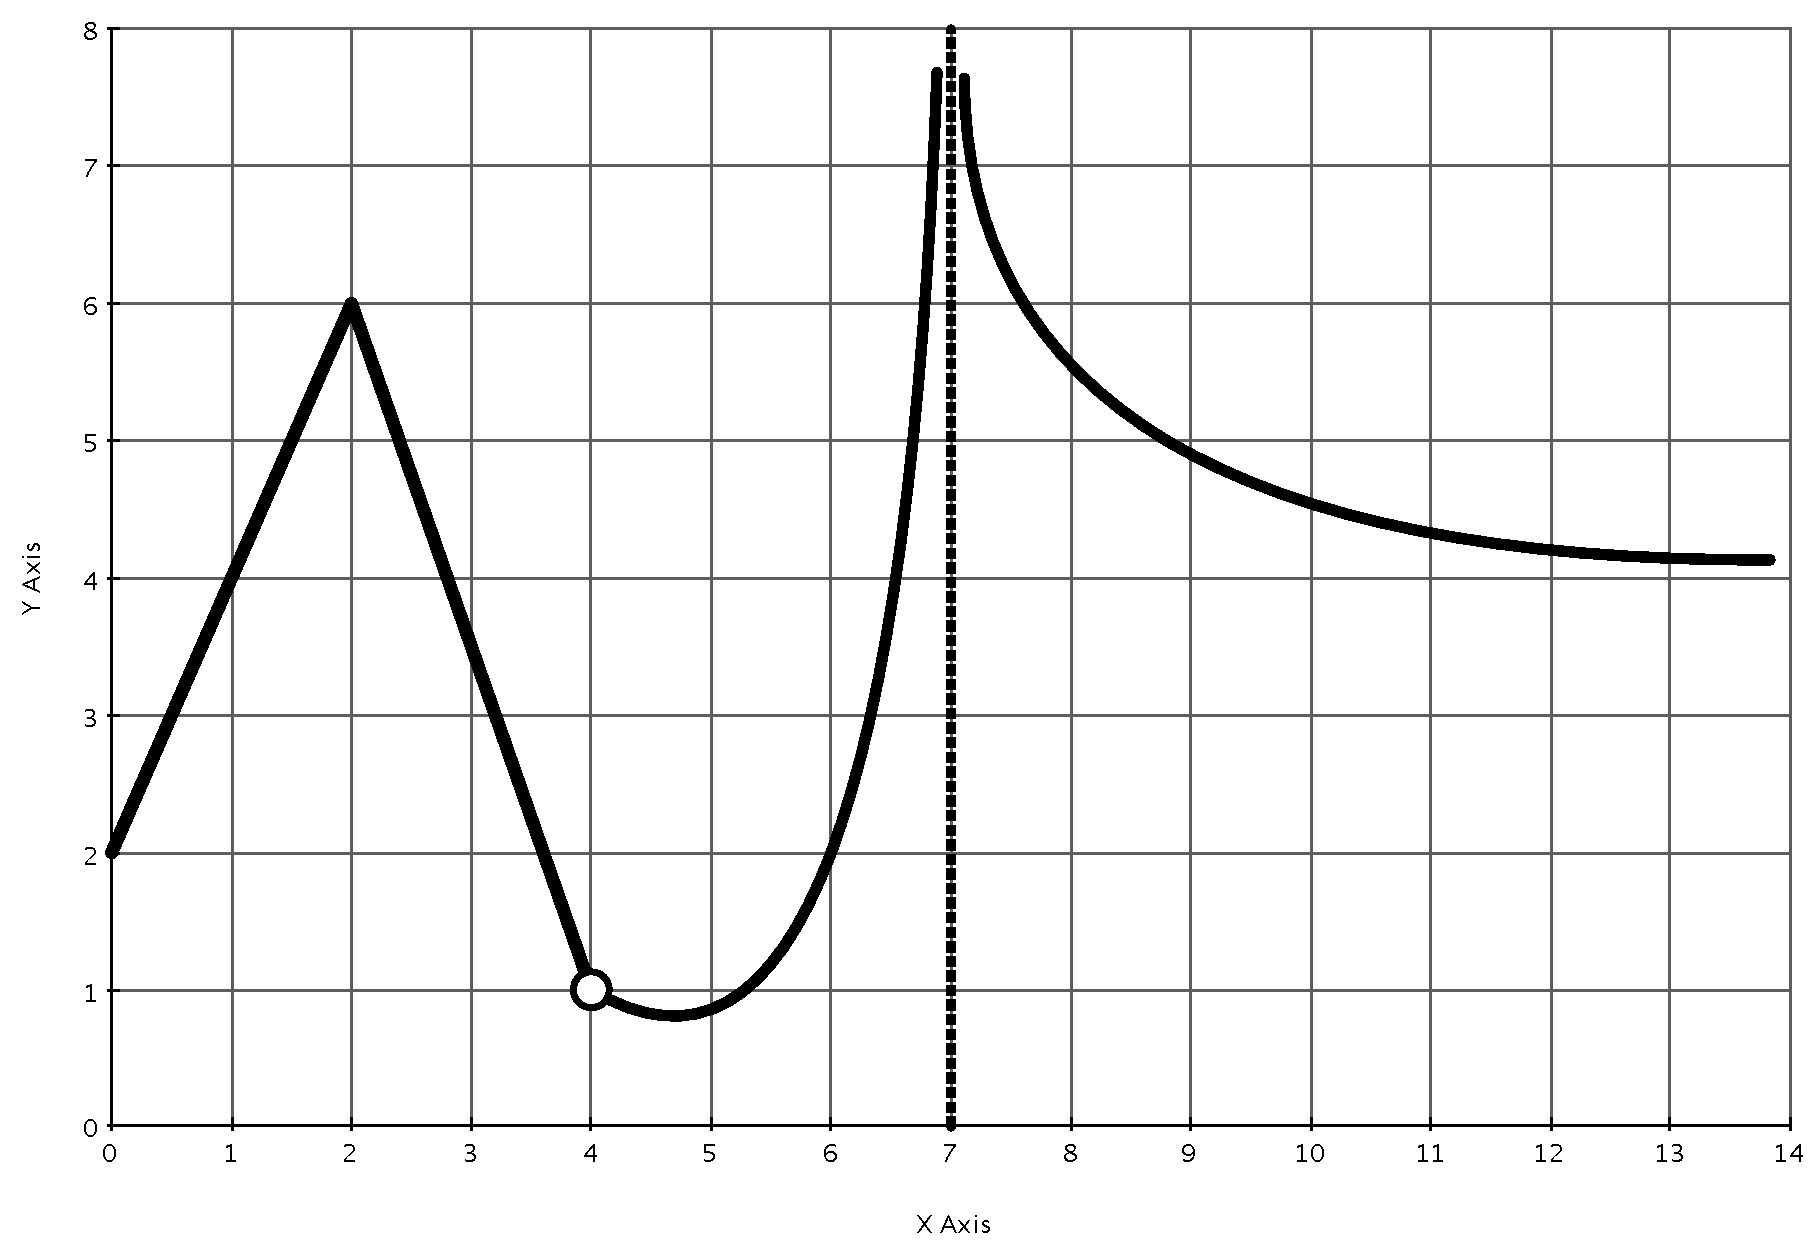
\includegraphics[width=0.35\textwidth]{fe-graphlimits}
\end{center}
	\begin{enumerate}
		\item State the value of $\displaystyle{\lim_{x \to 4} f(x)}$. If the limit fails to exist, say so. 
		\item State the value of $\displaystyle{\lim_{x \to 7^+} f(x)}$. If the limit fails to exist, say so. 		

		\item State the value of $\displaystyle{\lim_{x \to 2^-} f(x)}$. If the limit fails to exist, say so. 
		
		\item State the $x$-values of the points where $f$ is discontinuous. 
		
		
		\item State the $x$-values of the points where $f$ fails to be differentiable. 

			
	\end{enumerate}

	% \item Consider the function $h(t) = e^{-0.3t} \cos(t)$. Using a table of values with at least eight entries, evaluate $\displaystyle{\lim_{t \to 0} h(t)}$. 
\vspace{0.3in}

\noindent
\textbf{Problem 1.} Suppose the population, $P$, of China (in billions of people) can be approximated by the function $P(t) = 1.15(1.1014)^t$ where $t$ is the number of years since the start of 1993. 
	\begin{enumerate}
		\item Find the average rate of change in the population of China from 2000 to 2010. Show all work and include correct units on your answer. 
		\item Write a limit expression that, if evaluated, would give the exact instantaneous rate of change in the population of China on May 1, 2015. 
		\item Evaluate the limit expression in (b) to find the instantaneous rate of change in the population of China on May 1, 2015 using a table of values.  
	\end{enumerate}
\vspace{0.3in}

\noindent
\textbf{Problem 2 (CORE).} Consider the function $f(x) = 3x^2 - 5x + 10$. 
	\begin{enumerate}
		\item Find the equation for the tangent line to the graph of this function at $x = 5$. Use only the definition of the derivative. 
		\item Find the formula for the derivative of this function at any point. Use only the definition of the derivative. 
	\end{enumerate}

\vspace{0.3in}

\noindent
\textbf{Problem 3.} At a testing facility, a prototype electric car was monitored for performance as it drove down a straight track. Its position $s$, in meters from the starting point at time $t$ seconds, was measured using every $0.5$ seconds using a radar gun. The resulting data are given in a table: 
\begin{center}
		\begin{tabular}{c||ccccccccccccccc}
		$t$ & 0 & 0.5  & 1 & 1.5 & 2 & 2.5 & 3 & 3.5 & 4 & 4.5 & 5 & 5.5 & 6 & 6.5 & 7 \\ \hline
		$s$ & 0 & 5.2 & 9.1 & 12.3 & 16.1 & 20.8 & 31.5 & 35.2 & 40.2  & 45.3 & 51.1 & 64.3 & 70.2 & 79.0 & 80.3
		\end{tabular}
\end{center}
\begin{enumerate}
	\item Use difference estimates to construct a table for the car's velocity $v$ as a function of time. 
	\item Use a central difference estimate to estimate the car's acceleration at time $t = 4$. 
\end{enumerate}

\vspace{0.3in}

\noindent
\textbf{Problem 4.} For each of the following functions, use the algebraic rules for differentiation to perform the indicated tasks. 
	\begin{enumerate}
		\item $f(x) = x^2 + 3x - 7$; Find all the points where the tangent line to the graph of the function is horizontal. 
		\item $g(w) = 6w^4 + 7w^{2/3}$; Find the equation of the tangent line to the graph of the function when $w = 1$. 
		\item $s(t) = 3e^t - t^3$; If this function represents the position of a moving object, find the velocity and acceleration of the object when $t = 1$. The units of $t$ are seconds; the units of $s$ are feet.  
	\end{enumerate}

\vspace{0.3in}

\noindent
\textbf{Problem 5 (CORE).} For each of the following functions, use the algebraic rules for differentiation to perform the indicated tasks.
	\begin{enumerate}
		\item $f(x) = \dfrac{3x- 2}{4x - 9}$; Find the equation of the tangent line to the graph of the function when $x = 3$. 
		\item $g(t) = (t^3 + t^2 + t + 1)e^t$; Find formulas for the first and second derivatives. 
		\item $h(z) = \dfrac{z^4 + e^z}{z + 1}$; Find the exact value (no decimal approximations) of the slope of the tangent line to the graph of the function when $z = 5$. 
	\end{enumerate}


\vspace{0.3in}

\noindent
\textbf{Problem 6.} For each of the following functions, use the algebraic rules for differentiation to perform the indicated tasks. 
	\begin{enumerate}
		\item $y = \dfrac{\tan \theta}{\theta^2}$; Find formulas for the first, second, and third derivatives. 
		\item $y = e^\theta \sec \theta$; find an equation for the tangent line to this function when $\theta = \pi/4$. 
		\item $s(t) = 300 + 40 \sin (t)$; If this function represent the height ($s$, in meters) at time $t$ seconds of a weight oscillating up and down on the end of a spring, find the velocity and acceleration of the weight at $t = \pi/3$ seconds. 
	\end{enumerate}


\vspace{0.3in}

\noindent
\textbf{Problem 7 (CORE).} 
	\begin{enumerate}
		\item According to the U.S. standard atmospheric model, atmospheric temperature $T$ (in degrees Celsius), pressure $P$ (in kilopascals), and altitude $h$ (in meters) are related by the following formulas (valid whenever $h \leq 11000$):
		$$T = 15.04 - 0.000649h \qquad P = 101.29 + \left( \frac{T + 273.1}{288.08} \right)^{5.256}$$
		Use the Chain Rule to calculate a formula for $dP/dh$. Then find the instantaneous rate of change in atmospheric pressure with respect to altitude, at the point where $h = 3000$. 
		\item Consider the following table of data: 
		\begin{center}
			\begin{tabular}{c||c|c|c}
			$x$ & 1 & 4 & 6 \\ \hline
			$f(x)$ & 4 & 0 & 6 \\ 
			$g(x)$ & 5 & 7 & 4 \\
			$f'(x)$ & 4 & 1 & 6 \\
			$g'(x)$ & 5 & $1/2$ & 3
			\end{tabular}
		\end{center}
		Let $a(x) = f(g(x))$ and $b(x) = e^{f(x)}$. Calculate the values of $a'(6)$ and $b'(4)$. 
	\end{enumerate}


\vspace{0.3in}

\noindent
\textbf{Problem 8.} For each of the following functions, use the algebraic rules for differentiation to perform the indicated tasks. 
	\begin{enumerate}
		\item $f(t) = \ln(\sin t)$; Find an equation for the tangent line to the function when $t = \pi/4$. 
		\item $g(x) = \arcsin(e^x)$; Find the exact values (no decimal approximations) of the first and second derivative when $x = -1$
		\item The energy $E$ (in joules) radiated as seismic waves from an earthquake of Richter magnitude $M$ is given by the formula $\log_{10} E = 4.8 + 1.5M$. Express $E$ as a function of $M$; then find a formula for $dE/dM$ and find the instantaneous rate of change in energy when $M = 2$. 
 	\end{enumerate}


\vspace{0.3in}

\noindent
\textbf{Problem 9.} Consider the equation $x^3 - y^3 = 6xy$, which traces out the curve below: 
\begin{center}
	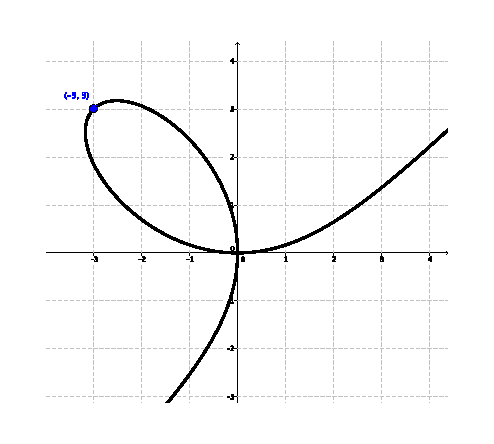
\includegraphics[width=0.35\textwidth]{a2-implicitplot2}
\end{center}

	\begin{enumerate}
		\item Find an equation for the line tangent to the curve at $(-3,3)$. Show all your work and do not merely estimate values from the graph. 
		\item From the graph you can see that there are two places where the tangent line to the curve is horizontal: at the origin, and at a point in the second quadrant. Find the exact coordinates of the one in the second quadrant. Show all work and make no estimations. 
	\end{enumerate}


\vspace{0.3in}

\noindent
\textbf{Problem 10 (CORE).} Consider the function 
$$f(t) = -\frac{1}{4} e^{-2t} (2t^2 + 2t - 9)$$
	\begin{enumerate}
		\item Find the exact values of all critical values of $f$. 
		\item Find the intervals on which $f$ is increasing and the intervals on which $f$ is decreasing. Show all work and do not merely estimate from a graph. 
		\item Classify each critical value you found as a local maximum, local minimum, or neither. Show all work and do not merely estimate from a graph. 
		\item Find all the intervals on which $f$ is concave up and all the intervals on which $f$ is concave down. Show all work and do not merely estimate from a graph. 
		\item Give the coordinates of all the inflection points of $f$. Show all work and do not merely estimate from a graph. 
	\end{enumerate}


\vspace{0.3in}

\noindent
\textbf{Problem 11.} For each of the following continuous functions, find the global minimum and global maximum value of the function on the given interval. 
	\begin{enumerate}
		\item $y = x^3 + 3x^2 - 9x + 2$, $[0,2]$
		\item $y = \sqrt{2} \theta - \sec \theta$, $[0, \pi/3]$
	\end{enumerate}


\vspace{0.3in}

\noindent
\textbf{Problem 12 (CORE).} 
	\begin{enumerate}
		\item A homeowner is putting up a pen area for his two dogs. The pen will be a rectangular fenced-in area, with a row of fence dividing the pen into two equal halves (one for each dog). He has enough money to afford 200 feet of fencing. What dimensions $x$ and $y$ of the fence maximize the area contained in the pens? 
		\item Find the point $(x,y)$ on the line $6x + y = 9$ that is closest to the point $(9, -5)$.  
	\end{enumerate}


\vspace{0.3in}

\noindent
\textbf{Problem 13.} 
	\begin{enumerate}
		\item An electrical voltage $V$ across a resistance $R$ generates an electrical current $I$ given by the formula $V = IR$.	If a constant voltage of 9 volts is put across a resistance that is increasing at a rate of 0.2 ohms per second when the resistance is 0.5 ohms, at what rate is the current changing?
		\item A hot air balloon rising vertically is tracked by an observer located 5 miles from the lift-off point. At a certain moment, the angle between the observer's line-of-sight and the horizontal is $\frac{\pi}{3}$ , and it is changing at a rate of 0.1 rad/min. How fast is the balloon rising at this moment?
	\end{enumerate}


\vspace{0.3in}

\noindent
\textbf{Problem 14.} At a testing facility, a prototype electric car was monitored for performance as it drove down a straight track. Its velocity $v$, in meters per second, at time $t$ seconds, was measured using every $0.5$ seconds using a radar gun. The resulting data are given in a table:
\begin{center}
	\begin{tabular}{c||ccccccccccccccc}
		$t$ & 0 & 0.5  & 1 & 1.5 & 2 & 2.5 & 3 & 3.5 & 4 & 4.5 & 5 & 5.5 & 6 & 6.5 & 7 \\ \hline
		$v$ & 0 & 10.2 & 22.1 & 29.3 & 34 & 35 & 35.1 & 35.2 & 34.3  & 25 & 21.1 &14.3 & 10.2 & 9 & 8.9
		\end{tabular} 		
\end{center} 
Estimate the distance that the car travelled over the entire $7$-second interval. Show work and put correct units on your answer.

\vspace{0.3in}

\noindent
\textbf{Problem 15  (CORE).} For each of the functions below, find the \emph{exact} value of the area between the graph of the function and the horizontal axis on the given interval. Show all work, and do not approximate.
	\begin{enumerate}
		\item $y = 3x^5 + x^2 - 2x$, $[0,4]$
		\item $y = 8/x^3$, $[4,9]$
		\item $y = \csc^2 x$, $[\pi/6, \pi/4]$
	\end{enumerate}





\end{document}